%tex_origin: ppt.tex
\section{Dual Stack Lite (DSL)}
\subsection{Métodos}

\begin{frame}
  \frametitle{Paquetes IPv4 bajo IPv6}
  \begin{columns}[t]
    \column{0.5\textwidth}
    	\begin{figure}
		\centering
		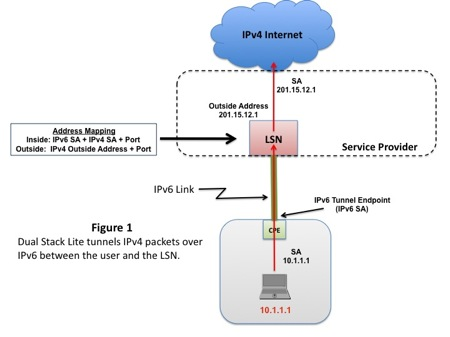
\includegraphics[width=150px]{img/img1.jpg}
	\end{figure}
    \column{0.5\textwidth}
    	\begin{itemize} %[itemsep=2em] 
		\footnotesize
		\item
			Cuando el cliente envía mensajes IPv4 se
			encapsulan en paquetes IPv6.
		\item
			En el LSN(Large Scale Nat) el paquete de 
			des-encapsula y NAT44 (Network address 
			translate for IPv4) actúa a continuación.
		\item
			La funcionalidad se implementa en el LSN.
		\item
			Para identificar cada equipo se realiza un mapeo
			que se guarda en una tabla con la siguiente 
			combinación: IPv6 address + IPv4 address + Port
	\end{itemize}
  \end{columns}
\end{frame}

\begin{frame}
  \frametitle{Paquetes IPv4 bajo IPv6 - Generalización}
  \begin{columns}[t]
    \column{0.5\textwidth}
    	\begin{figure}
		\centering
		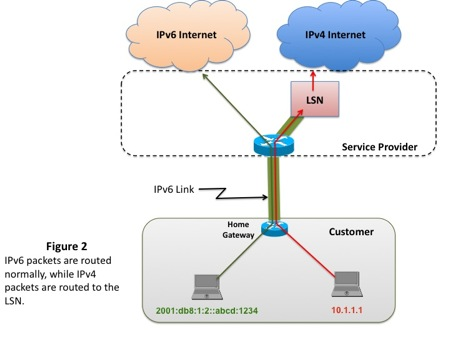
\includegraphics[width=150px]{img/img2.jpg}
	\end{figure}
    \column{0.5\textwidth}
	 \begin{itemize}
		\item
			Un mensaje IPv6 se envía normalmente.
		\item
			Si el mensaje va en IPv4 se utiliza la 
			técnica mencionada anteriormente. Es decir, 
			el paquete IPv4 encapsulado en uno IPv6 y 
			enviado a un LSN disponible.
	\end{itemize}
  \end{columns}
\end{frame}

\begin{frame}
  \frametitle{Problemas}
  	\begin{itemize}[itemsep=2em]
		\item
			La funcionalidad que permite el paso de mensajes
			en IPv4 a través de IPv6 debe ser implementada
			en los equipos locales.
		\item
			En general las ISP son reacias a molestar a los
			usuarios, por lo que la estrategia consistiría
			en implementar el método en los nuevos clientes
			y a medida que se renueven los equipos.
	\end{itemize}
\end{frame}

\begin{frame}
  \frametitle{Esquema ideal}
  \begin{columns}[t]
    \column{0.5\textwidth}
    	\begin{figure}
		\centering
		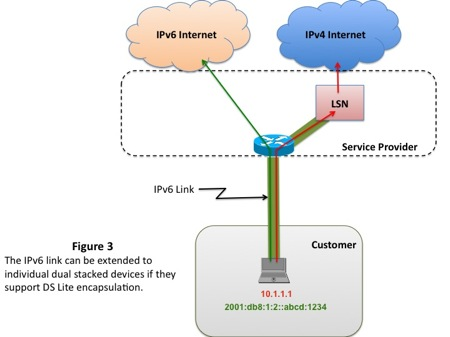
\includegraphics[width=150px]{img/img3.jpg}
	\end{figure}
    \column{0.5\textwidth}
    	\begin{itemize}[itemsep=2em]
		\item
			Dual Stack implementado en los equipos.
		\item
			Los equipos son capaces de interactuar
			con ambos protocolos.
	\end{itemize}
  \end{columns}
\end{frame}





